%versi 3 (22-07-2020)
\chapter{Landasan Teori}
\label{chap:teori}

\section{BigQuery\cite{bqa, bqIntroduction}}
Google memiliki salah satu produk yaitu BigQuery yang berbasis \textit{cloud} dan dapat digunakan untuk menganalisis data tanpa harus memikirkan database. BigQuery memaksimalkan fleksibelitas dengan memisahkan memisahkan mesin komputasi yang menganalisa data. BigQuery dapat digunakan sebagai tempat penyimpanan dan data tersebut dapat dianalisis. Google meluncurkan BigQuery secara publik pada tahun 2012. Saat ini BigQuery sudah berkembang menjadi penyedia penyimpanan terstruktur berbasis \textit{cloud} yang dikelola dan dihosting. 

\subsection{\textit{Cloud Storage System}}
Selain sebagai tempat untuk menjalankan \textit{query} dari data, saat ini BigQuery juga merupakan tempat penyimpanan data terstruktur di \textit{cloud}. Data akan direplikasi ke beberapa lokasi yang berbeda secara geografis untuk meningkatkan ketersediaan dan ketahanan. Jika pusat data di Google pada suatu lokasi ditutup, data tetap dapat diakses tanpa terjadi gangguan. Data juga akan direplikasi dalam sebuah kluster agar tidak terjadi kehilangan data jika terjadi kegagalan perangkat keras. 

\subsection{\textit{SQL (Structured Query Language) \cite{book:22611}}}
SQL adalah bahasa pemograman menghasilkan, memanipulasi, dan mengambil informasi dari database relasional. Mengambil informasi dari database relasional harus menggunakan \textit{query}. \textit{Query} merupakan sintaks atau perintah yang digunakan untuk mengambil dan menghasilkan data dari database. Terdapat beberapa komponen atau klausa dari \textit{query} yang digunakan mengambil dan menghasilkan data dari database dapat dilihat pada tabel \ref{table:query_clause}

\begin{table}[h!]
	\centering
	\begin{tabular}{|l|l|} 
		\hline
		\textbf{Clause Name} & \textbf{Purpose} \\
		\hline
		Select & Menentukan kolom dari suatu tabel yang akan ditampilkan dalam \textit{query result}\\
		\hline
		From & Mengidentifikasi tabel yang ingin diambil datanya\\
		\hline
		Where & Membatasi jumlah baris dalam \textit{query result}\\
		\hline
		Group by & Mengelompokkan baris berdasarkan nilai kolom yang sama\\
		\hline
		Having & Membatasi jumlah baris dalam \textit{query result} menggunakan data yang dikelompokkan\\
		\hline
		Order by & Mengurutkan \textit{query result} berdasarkan satu atau lebih kolom\\
		\hline
	\end{tabular}
	\caption{\textit{Query Clauses}}
	\label{table:query_clause}
\end{table}

Didalam \textit{query} juga terdapat beberapa fungsi agregat untuk melakukan operasi tertentu yang dapat dilihat pada tabel \ref{table:agg_func}
\begin{table}[h!]
	\centering
	\begin{tabular}{|l|l|} 
		\hline
		\textbf{Aggregate Function} & \textbf{Purpose} \\
		\hline
		Max() & Mengembalikan nilai maksimal dari atribut sebuah tabel\\
		\hline
		Min() & Mengembalikan nilai minimum dari atribut sebuah tabel\\
		\hline
		Avg() & Mengembalikan nilai rata-rata dari atribut sebuah tabel\\
		\hline
		Sum() & Mengembalikan jumlah nilai dari atribut sebuah tabel\\
		\hline
		Count() & Mengembalikan jumlah baris dari atribut sebuah tabel\\
		\hline
	\end{tabular}
	\caption{\textit{Aggregate Function}}
	\label{table:agg_func}
\end{table}

\subsubsection{Querying Multiple Tables}
Karena database relasional di-\textit{design} dibentuk dengan mengamanatkan bahwa setiap entitas dibuat kedalam tabel yang terpisah, sehingga dibutuhkan mekanisme untuk menghubungkan beberapa tabel dalam \textit{query} yang sama. Mekanisme ini disebut dengan join. Terdapat beberapa jenis join sebagai berikut:
\begin{itemize}
	\item LEFT OUTER JOIN \\
	Kata kunci kiri menunjukkan bahwa tabel di sisi kiri klausa from bertanggung jawab untuk menentukan jumlah baris dalam kumpulan hasil, sedangkan tabel di sisi kanan digunakan untuk memberikan nilai kolom setiap kali ditemukan kecocokan.
	\item RIGHT OUTER JOIN \\
	Kata kunci kiri menunjukkan bahwa tabel di sisi kanan klausa from bertanggung jawab untuk menentukan jumlah baris dalam kumpulan hasil, sedangkan tabel di sisi kiri digunakan untuk memberikan nilai kolom setiap kali ditemukan kecocokan.
	\item FULL OUTER JOIN \\
	Full outer join merupakan gabungan dari left outer join dan right outer join.
	\item CROSS JOIN \\
	Cross join menggabungkan beberapa tabel dengan cara mengkali silangkan tabel tersebut tanpa menentukan kondisi apapun.
	\item INNER JOIN \\
	Inner join menghubungkan dua atau lebih tabel dengan hubungan antara dua kolom.
\end{itemize}

\subsubsection{Subquery}
\textit{Subquery} merupakan query yang yang terkandung dalam \textit{query} lain. Sebuah \textit{subquery} selalu diapit dalam tanda kurung, dan biasanya dieksekusi terlebih dahulu sebelum \textit{query} yang memuatnya. Tabel yang dikembalikan oleh \textit{subquery} menentukan bagaimana tabel tersebut dapat digunakan dan operator mana yang dapat digunakan oleh \textit{query} yang memuatnya untuk berinteraksi dengan tabel yang dikembalikan oleh \textit{subquery}. Ketika query yang memuat telah selesai dieksekusi, tabel yang dikembalikan oleh subquery akan dibuang, membuat subquery bertindak seperti tabel sementara dengan cakupan pernyataan. 


\section{HTTP Archive \cite{httparchiveAbout}}
HTTP Archive adalah sebuah \textit{open-source project} yang melihat bagaimana website dibuat. HTTP Archive menyediakan data-data historis untuk melihat bagaimana website berkembang. HTTP Archive pertama sekali dimulai pada tahun 2010 oleh Steve Souders dan di-\textit{maintain} oleh Pat Meenan, Rick Viscomi, Paul Calvano, and Barry Pollard. HTTP Arhive memiliki keterbatasan seperti HTTP Archive hanya melihat halaman utama. Misalnya sebagian besar \textit{website} terdiri dari banyak halaman web terpisah. Karena batasan ini sehingga ada kemungkinan bahwa suatu halaman yang dianalisis tidak mewakili sebuah situs website. Di dalam HTTP Archive terdapat dataset yang dapat diambil menggunakan teknologi BigQuery, dataset tersebut adalah sebagai berikut:
\begin{enumerate}
	\item almanac\\
	\item blink$\_$features\\
	\item core$\_$web$\_$vitals\\
	\item latest\\
	\item lighthouse\\
	Dataset pada lighthouse berisi tabel-tabel dari bulan Juni tahun 2017 sampai dengan sekarang yang terdiri dari website pada mobile. Dataset bulan Agustus tahun 2020 baris pada mobile memiliki 6.290.147 baris \ref{fig:ct_lh_mobile} yang dapat dianalisis. Masing-masing terdiri dari URL dan report. \textit{URL (Uniform Resource Locator)} merupakan nama-nama domain dan \textit{report}
	\begin{figure}[H]
		\centering  
		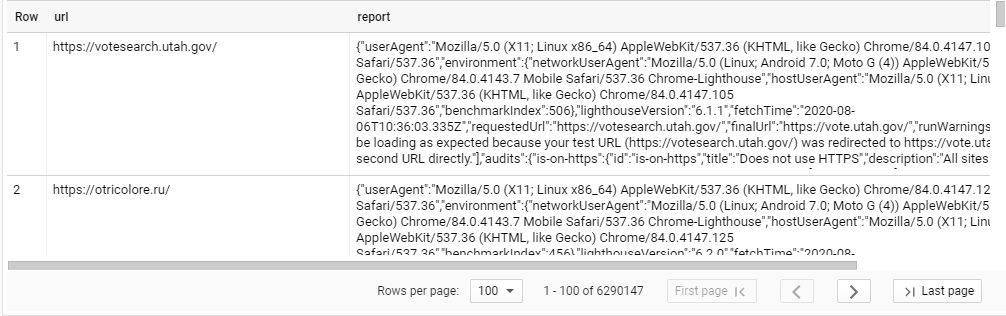
\includegraphics[scale=0.9]{Gambar/2020_08_01_mobile_jumlah_baris_lighthouse.PNG}  
		\caption{Jumlah baris pada tabel lighthouse di mobile} 
		\label{fig:ct_lh_mobile} 
	\end{figure}
	
	\item pages\\
	Dataset pada pages berisi tabel-tabel dari bulan Januari tahun 2016 sampai dengan sekarang yang terdiri dari website pada desktop dan mobile. Dataset bulan Agustus tahun 2020 baris pada desktop memiliki 5.593.642 baris \ref{fig:ct_pages_desktop} dan pada mobile memiliki 6.347.640 baris \ref{fig:ct_pages_mobile} yang dapat dianalisis. Masing-masing terdiri dari URL dan payload. \textit{URL (Uniform Resource Locator)} merupakan nama-nama domain dan \textit{payload}
	\begin{figure}[H]
		\centering  
		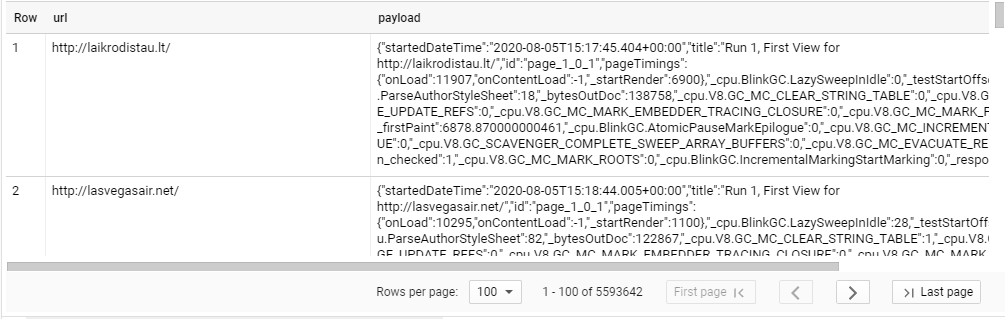
\includegraphics[scale=0.9]{Gambar/2020_08_01_desktop_jumlah_baris_pages.PNG}  
		\caption{Jumlah baris pada tabel pages di desktop} 
		\label{fig:ct_pages_desktop} 
	\end{figure}
	
	\begin{figure}[H]
		\centering  
		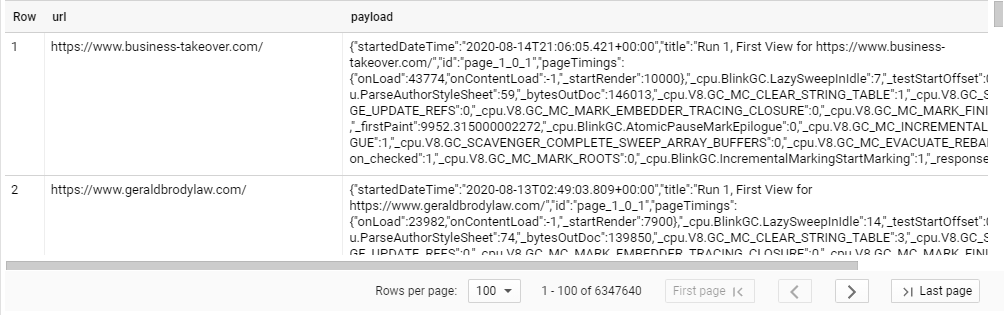
\includegraphics[scale=0.9]{Gambar/2020_08_01_mobile_jumlah_baris_pages.PNG}  
		\caption{Jumlah baris pada tabel pages di mobile} 
		\label{fig:ct_pages_mobile} 
	\end{figure}
	
	\item requests\\
	Dataset pada request berisi tabel-tabel dari bulan Januari tahun 2016 sampai dengan sekarang yang terdiri dari website pada desktop dan mobile. Dataset bulan Agustus tahun 2020 baris pada desktop memiliki 535.841.778 baris dan pada mobile memiliki 579.752.745 baris yang dapat dianalisis. Masing-masing terdiri dari URL dan payload. \textit{URL (Uniform Resource Locator)} merupakan nama-nama domain dan \textit{payload}.
	\item response$\_$bodies\\
	Dataset pada response$\_$bodies berisi tabel-tabel dari bulan Januari tahun 2016 sampai dengan sekarang yang terdiri dari website pada desktop dan mobile. Dataset bulan Agustus tahun 2020 baris pada desktop memiliki 215.621.667 baris dan pada mobile memiliki 270.249.686 baris yang dapat dianalisis. Masing-masing terdiri dari page, URL, body, truncated, dan requestId.
	\item sample$\_$data\\
	\item sample$\_$data$\_$2020\\
	\item scratchspace\\
	\item summary$\_$pages\\
	Dataset pada summary$\_$pages berisi tabel-tabel dari bulan November tahun 2010 sampai dengan sekarang yang terdiri dari website pada desktop dan mobile. Dataset bulan Agustus tahun 2020 baris pada desktop memiliki 5.593.642 baris dan pada mobile memiliki 6.347.919 baris yang dapat dianalisis. Masing-masing terdiri dari pageid, createDate, archive, label, crawlid, wptid, wptrun, url, urlShort, urlhash, cdn, startedDateTime, TTFB, renderStart, onContentLoaded, onLoad, fullyLoad, visualComplete, PageSpeed, SpeedIndex, rank, reqTotal, reqHTML, reqJS, reqCSS, reqImg, reqGif, reqJpg, reqPng, reqFont, reqFlash, reqJson, reqOther, bytesTotal, bytesHTML, bytesJS, bytesCSS, bytesImg, bytesGif, bytesJpg, bytesPng, bytesFont, bytesFlash, bytesJson, bytesOther, bytesHtmlDoc, numDomains, maxDomainReqs, numRedirects, numErrors, numGlibs, numHttps, numCompressed, numDomElements, maxageNull, maxage0, maxage1, maxage30, maxage365, maxageMore, gzipTotal, gzipSavings, $\_$connections, $\_$adult$\_$site, avg$\_$dom$\_$depth, document$\_$height, document$\_$width, localstorage$\_$size, sessionstorage$\_$size, num$\_$iframes, num$\_$scripts, doctype, meta$\_$viewport, reqAudio, reqVideo, reqText, reqXml, reqWebp, reqSvg, bytesAudio, bytesVideo, bytesText, bytesXml, bytesWebp, bytesSvg, num$\_$scripts$\_$async, num$\_$scripts$\_$sync, usertiming.
	\item summary$\_$requests\\
	Dataset pada response$\_$requests berisi tabel-tabel dari bulan November tahun 2010 sampai dengan sekarang yang terdiri dari website pada desktop. Dataset bulan Agustus tahun 2020 baris pada desktop memiliki 215.621.667 baris dan pada mobile memiliki 1.234.599 baris yang dapat dianalisis. Masing-masing terdiri dari requestid, pageid, startedDateTime, time, method, url, urlShort, redirectUrl, firstReq, firstHtml, reqHttpVersion, reqHeaderSize, reqBodySize, reqCookieLen, reqOtherHeader, status, respHttpVersion, respHeaderSize, respBodySize, respSize, respCookieLen, expAge, mimeType, respOtherHeader, req$\_$accept, req$\_$accept$\_$charset, req$\_$accept$\_$encoding, req$\_$accept$\_$language, req$\_$connection, req$\_$host, req$\_$if$\_$modified$\_$since, req$\_$if$\_$none$\_$match, req$\_$referer, req$\_$user$\_$agent, resp$\_$accept$\_$ranges, resp$\_$age, resp$\_$cache$\_$control, resp$\_$connection, resp$\_$content$\_$encoding, resp$\_$content$\_$language, resp$\_$content$\_$length, resp$\_$content$\_$location, resp$\_$content$\_$type, resp$\_$date, resp$\_$etag, resp$\_$expires, resp$\_$keep$\_$alive, resp$\_$last$\_$modified, resp$\_$location, resp$\_$pragma, resp$\_$server, resp$\_$transfer$\_$encoding, resp$\_$vary, resp$\_$via, resp$\_$x$\_$powered$\_$by.
	\item technologies\\
	Dataset pada technologies berisi tabel-tabel dari bulan Januari tahun 2016 sampai dengan sekarang yang terdiri dari website pada desktop dan mobile. Dataset bulan Agustus tahun 2020 baris pada desktop memiliki 61.203.638 baris  dapat dilihat pada gambar \ref{fig:ct_tech_desktop} dan pada mobile memiliki 67.452.994 baris \ref{fig:ct_tech_mobile} yang dapat dianalisis. Masing-masing terdiri dari 4 kolom yaitu \textit{URL}, \textit{category}, \textit{app}, \textit{info}. Pada kolom \textit{URL (Uniform Resource Locator)} merupakan nama-nama domain, \textit{category} merupakan jenis aplikasi yang digunakan pada website tersebut, \textit{app} merupakan aplikasi yang digunakan website tersebut, \textit{info} merupakan informasi tambahan dari aplikasi. 
	
	\begin{figure}[H]
		\centering  
		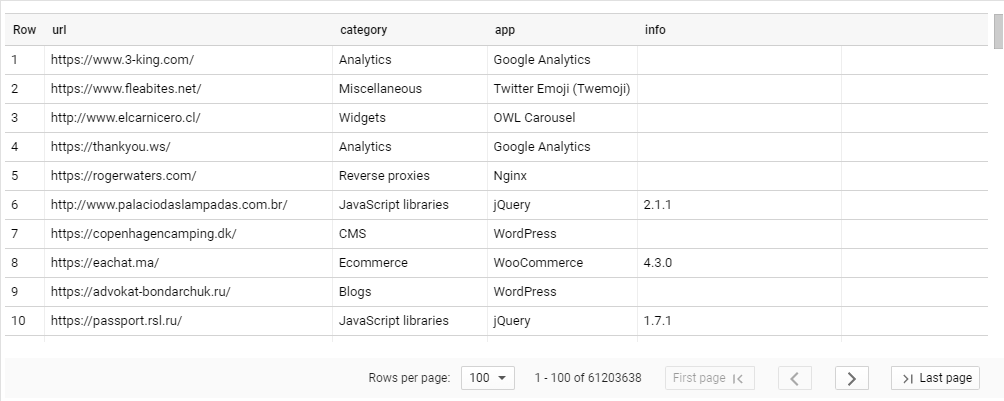
\includegraphics[scale=0.9]{Gambar/2020_08_01_desktop_jumlah_baris.PNG}  
		\caption{Jumlah baris pada tabel technologies di desktop} 
		\label{fig:ct_tech_desktop} 
	\end{figure}
	
	\begin{figure}[H]
		\centering  
		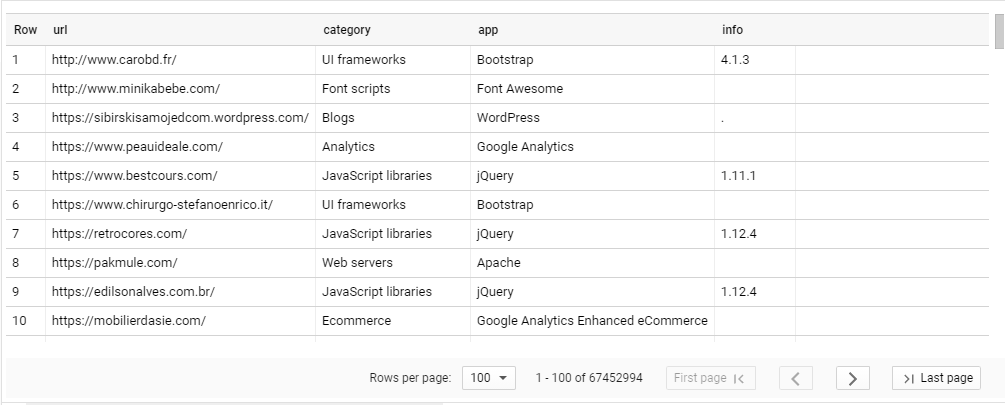
\includegraphics[scale=0.9]{Gambar/2020_08_01_mobile_jumlah_baris.PNG}  
		\caption{Jumlah baris pada tabel technologies di mobile} 
		\label{fig:ct_tech_mobile} 
	\end{figure}
	
	\item urls\\
	\item wappalyzer\\
\end{enumerate}


\section{Web Almanac \cite{webalmanacMetho}}
Web Almanac adalah sebuah projek yang dikelola oleh HTTP Archive. Misi web almanac adalah menggabungkan statistik mentah dan tren HTTP Archive dengan keahlian komunitas web. Semua metrik yang disediakan oleh web almanac dapat direproduksi secara publik menggunakan dataset di BigQuery. Kueri dapat ditelusuri dengan menggunakan semua bab di repositori GitHub web almanac yang dapat dilihat pada \footnote{https://github.com/HTTPArchive/almanac.httparchive.org/tree/main/sql/2020}: 
\begin{enumerate}
	\item Accessibility\\
	Aksesibilitas web adalah tentang pencapaian fitur dan informasi serta memberikan akses lengkap ke semua aspek antarmuka bagi orang yang tidak memiliki akses. Sebuah produk digital atau situs web tidak lengkap jika tidak dapat digunakan oleh semua orang. 
	\item Caching\\
	Caching adalah teknik yang memungkinkan penggunaan kembali konten yang diunduh sebelumnya. Caching melibatkan sesuatu seperti server atau web browser untuk menyimpan konton dan menandainya agar dapat digunakan kembali.
	\item Capabilities\\
	Capabilties memberikan \textit{overview} tentang berbagai API web modern. Hal ini penting untuk menjaga web tetap relevan sebagai platform. 
	\item CMS\\
	Istilah CMS mengacu pada sistem yang memungkinkan individu dan organisasi untuk membuat, mengelola, dan mempublikasikan konten. CMS pada konton web adalah sistem yang bertujuan untuk membuat, mengelola, dan menerbitkan konten untuk dikonsumsi dan dialami melalui internet.
	\item Compression\\
	Menggunakan HTTP Compression membuat pemuatan situs lebih cepat dan menjamin pengalaman penggunaan yang lebih baik. Penggunaan compression yang efektif dapat mengurangi berat halaman dan meningkatkan kinerja web.
	\item CSS\\
	CSS adalah bahasa yang digunakan untuk membuat tampilan dan format pada web dan media lainnya.
	\item Ecommerce\\
	Ecommerce platform adalah perangkat lunak atau layanan yang memungkinkan untuk membuat dan mengoperasikan sebuah toko online.
	\item Fonts\\
	Fonts adalah bagian penting dalam sebuah situs web dan tipografi adalah seni menyajikan teks tersebut dengan cara yang menarik dan efektif secara visual. Dalam pembuatan tipografi yang baik dibutuhkan pemilihan font yang sesuai. Dalam hal ini akan ditunjukkan bagaimana font web digunakan dan bagaimanafont tersebut dioptimalkan. 
	\item HTTP\\
	HTTP adalah protokol lapisan aplikasi yang dirancang untuk mentransfer informasi antara perangkat jaringan dan berjalan di atas lapisan lain dari tumpukan protokol jaringan. Dalam web almanac akan mengulas bagaimana status penerapan HTTP/2 atau HTTP versi dua pada saat ini.
	\item Jamstack\\
	Jamstack adalah konsep arsitektur yang relatif baru yang dirancang untuk membuat web lebih cepat, lebih aman, dan lebih mudah untuk diskalakan. Dalam web almanac akan memperkirakan dan menganalisis pertumbuhan situs Jamstack, kinerja kerangka kerja Jamstack populer, serta analisis pengalaman pengguna nyata menggunakan metrik Core Web Vitals.
	\item Javascript\\
	JavaScript adalah bahasa pemograman yang digunakan untuk menentukan perilaku. 
	\item Markup\\
	HTML adalah dasar dari sebuah website yang akan ditampilkan ke-\textit{user}. Dalam web almanac mengacu pada kumpulan halaman \textit{mobile}.
	\item Media\\
	Pada web alamanac, media digunakan untuk menganalisa bagaimana menggunakan gambar dan video di web.
	\item Mobile-web\\
	Saat ini, mobile-web sudah menjadi cara utama banyak orang untuk mengakses website. Dalam mobile-web akan terlihat tren saat ini pada mobile-web.
	\item Page-weight\\
	Page-weight adalah salah satu metrik sederhana yang tersedia. Memuat sebuah halaman akan memberikan gambaran tentang ukuran dari \textit{resource} yang diambil atau di-\textit{request}.    \item Performance\\
	Dalam web almanac, akan melihat data kinerja di dunia nyata yang disediakan oleh Laporan Pengalaman Pengguna Chrome (CrUX) melalui lensa perkembangan baru tersebut serta menganalisis beberapa metrik relevan lainnya.
	\item Privacy\\
	Web almanac memberikan gambaran umum tentang keadaan privasi saat ini di web. Hal ini bertujuan untuk meningkatkan akuntabilitas pemroses data dan transparansi mereka terhadap pengguna. Dalam hal ini, kami membahas prevalensi pelacakan online dengan berbagai teknik dan tingkat adopsi spanduk persetujuan cookie dan kebijakan privasi oleh situs web.
	\item PWA\\
	Dalam web almanac, kita akan melihat setiap komponen yang membuat PWA seperti apa adanya, dari perspektif berbasis data.
	\item Resource-hints\\
	
	\item Security\\
	Dalam web almanac, akan dilakukan menganalisis penerapan berbagai fitur keamanan secara mendalam dan dalam skala besar, kami mengumpulkan wawasan tentang berbagai cara pemilik situs web menerapkan mekanisme keamanan ini, didorong oleh insentif untuk melindungi penggunanya.
	\item SEO\\
	Dalam web almanac, untuk mengidentifikasi dan menilai elemen dan konfigurasi utama yang berperan dalam pengoptimalan pencarian organik situs web.
	\item Third-parties\\
	Web almanac meninjau prevalensi konten pihak ketiga dan bagaimana hal ini telah berubah sejak 2019.
\end{enumerate}



\section{OSEMN Framework}
OSEMN merupakan data science framework yang memberikan langkah-langkah pengerjaan proyek.\footnote{https://towardsdatascience.com/5-steps-of-a-data-science-project-lifecycle-26c50372b492}
\subsection{Obtain Data}
Obatain data berarti mengumpulkan data dari berbagai sumber. Langkah ini adalah langkah pertama. Mengumpulkan data sangat penting karena dalam melakukan sebuah proyek harus memiliki data. Data dapat didapat dengan meng-query dari database.

\subsection{Scrub Data}
Pada proses scrubbing data, data yang dikumpulkan tersebut akan dibersihkan atau difilter. Jika menggunakan data yang tidak difilter maka akan mempengaruhi keakuratan hasil akhir. Scrubbing data bisa saja merupakan ekstraksi data dan bertukar nilai.

\subsection{Explore Data}
Pada explore data, akan dilakukan pengecekan terhadap tipe dari data. Kemudian data-data tersebut akan dikumpulkan dan dibandingkan sehingga mendapat kesimpulan dari data yang ingin dicari. 

\subsection{Model Data}
Model data adalah pembuatan hasil akhir dari data yang diselidiki. Tujuan dari model data adalah mengelompokan data untuk memahami logika di balik cluster tersebut. 

\subsection{Interpreting Data}
Interpreting data mengacu pada penyajian data, penyampaian hasil agar dapat menunjukkan kesimpulan. Hasil-hasil yang ditunjukkan dapat berupa grafik-garfik agar dapat dijelaskan secara jelas dan aplikatif.




\section{Pengukuran Aplikasi Usang Pada Beberapa Website Populer Di Indonesia\cite{pascal}}
Pada bagian ini akan dijelaskan tentang research method dan hasil keseluruhan dari \cite{pascal}.
\subsection{\textit{Research Method}}
\begin{enumerate}
	\item Memilih list website yang populer\\
	Memilih website paling populer dilakukan dengan mengambil daftar dari website teratas dari Alexa dengan negara tertentu.
	\item Mengidentifikasi aplikasi yang dipakai website\\
	Untuk setiap website akan dilakukan pengidentifikasian nomor versi yang dipakai. Hal ini dibantu dengan menggunakan \textit{third party} yaitu Wappalyzer. 
	\item Mengelompokkan berdasarkan nama aplikasi dan ambil versi yang didukung\\
	Untuk melihat nomor versi yang masih didukung akan dilakukan pencarian di website resmi dari setiap aplikasi. Terdapat beberapa website yang tidak dapat ditampilkan versinya, sehingga suatu website dapat didefinisikan didukung jika memenuhi kondisi sebagai beikut:
	\begin{itemize}
		\item Versi aplikasi yang didukung dapat dilihat secara eksplisit di dalam website.
		\item Dokumen untuk versi aplikasi tersebut masih tersedia.
		\item Aplikasi secara langsung memberikan pernyataan untuk versi yang masih didukung.
	\end{itemize}
	
	\item Membandingkan versi yang dipakai aplikasi saat ini dengan versi aplikasi yang didukung dapat dilihat pada gambar \ref{fig:apr}\\
	Buka kembali setiap aplikasi kemudian menggunakan Wappalyzer untuk membandingkan versi aplikasi yang dipakai dengan versi aplikasi yang masih didukung. Klasifikasikan setiap aplikasi di setiap situs web menjadi salah satu dari berikut ini:
	\begin{itemize}
		\item \textit{Not-versioned} berarti aplikasi yang terdeteksi oleh Wappalyzer tidak memiliki informasi versi sehingga tidak dapat dibandingkan.
		\item Non-konklusif dapat berarti salah satu dari dua:
		\begin{itemize}
			\item Dapat mengambil nomor versi yang digunakan dalam aplikasi, tetapi kami tidak dapat menentukan apakah versi tersebut masih didukung atau tidak oleh pengelola.
			\item Versi yang didukung untuk aplikasi tertentu tidak diketahui.
		\end{itemize}
		\item Tidak didukung berarti dapat disimpulkan bahwa aplikasi yang digunakan menggunakan nomor versi yang tidak didukung oleh pengelola.
		\item Didukung berarti dapat disimpulkan bahwa aplikasi yang digunakan menggunakan nomor versi masih didukung oleh pengelola.
	\end{itemize}
	\begin{figure}[H]
		\centering  
		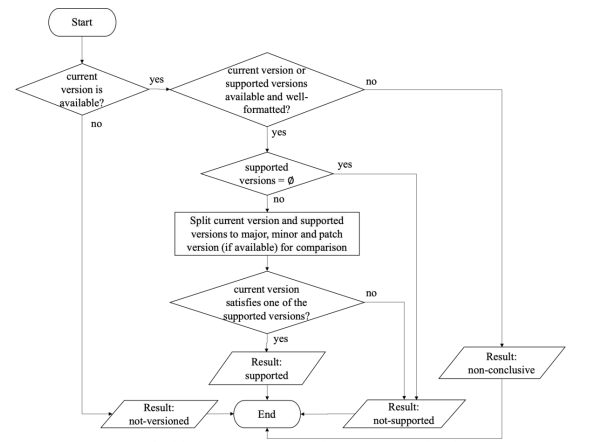
\includegraphics[scale=0.9]{Gambar/compare_version.PNG}  
		\caption{\textit{ Algorithm to compare current version versus supported versions}} 
		\label{fig:apr} 
	\end{figure}
\end{enumerate}


\subsection{\textit{Hasil Keseluruhan}}
Pada paper\cite{pascal}, dari 1.500 URL yang dideteksi oleh Wappalyzer, hanya 1.439 URL yang berhasil diidentifikasi. Dari 1.500 URL terebut ditemukan total 12.762 aplikasi yang dapat dilihat pada tabel \ref{table:apr}
\begin{table}[h!]
	\centering
	\begin{tabular}{lrr} 
		\hline
		\textbf{Result} & \textbf{Application count} & \textbf{Percentage}\\
		\hline
		Not-versioned & 8,980 & 70.37\\
		Non-conclusive & 1,409 & 11.04\\
		Unsupported & 1,508 & 11.82\\
		Supported & 865 & 6.78\\
		\hline
		Total & 12,762 & 100.00\\
		\hline
		
	\end{tabular}
	\caption{Overall application count for measurement result}
	\label{table:apr}
\end{table}











